\documentclass{beamer}
\usepackage[utf8]{inputenc}

\usetheme{CambridgeUS}
\usecolortheme{default}
\usepackage{tikz}

%------------------------------------------------------------
%This block of code defines the information to appear in the
%Title page
\title[Master Thesis] %optional
{Advancing Packet-Level Predictions with Transformers}

\author[Siddhant Ray] % (optional)
{Siddhant Ray}

\institute[ETH Zürich] % (optional)
{
  Dept. of Information Technology and Electrical Engineering(D-ITET) \\
  ETH Zürich
}

\date[September 2022] % (optional)

\titlegraphic{
    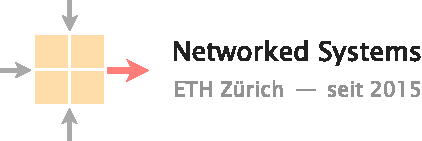
\includegraphics[width=2cm]{figures/nsg_logo.pdf}
    \hspace{2cm}
     
\includegraphics[width=2cm]{figures/eth_logo.pdf}
}

%End of title page configuration block
%------------------------------------------------------------



%------------------------------------------------------------
%The next block of commands puts the table of contents at the 
%beginning of each section and highlights the current section:

%\AtBeginSection[]
%{
%  \begin{frame}
 %   \frametitle{Table of Contents}
 %   \tableofcontents[currentsection]
 % \end{frame}
%}
%------------------------------------------------------------


\begin{document}

%The next statement creates the title page.
\frame{\titlepage}


%---------------------------------------------------------
%This block of code is for the table of contents after
%the title page
%\frametitle{Table of Contents}
%
%end{frame}
%---------------------------------------------------------


\section{Motivation}

%---------------------------------------------------------
%Changing visivility of the text
\begin{frame}
\frametitle{Why Transformers?}

Show vision figure here.

\begin{itemize}
    \item<1-> Efficient learning with attention
    \item<1-> Data availability
    \item<2-> Re-use, don't re-train from scratch
    \item<2-> Fine-tune for specific tasks
    \end{itemize}
\end{frame}

%---------------------------------------------------------


%---------------------------------------------------------
%Example of the \pause command
\begin{frame}
\frametitle{Success in CV and NLP}
Show \pause
examples.
\end{frame}
%---------------------------------------------------------

\section{Design}

%---------------------------------------------------------
%Highlighting text
\begin{frame}
\frametitle{NTT architecture}
Show architecture. \pause

\alert{highlight} stuff because it's important.
Not too much. \pause 

\begin{block}{Remark}
Use block if needed
\end{block}
\pause

\begin{alertblock}{Important theorem}
Alert probably not needed.
\end{alertblock}
\pause

\begin{examples}
Some examples?
\end{examples}
\end{frame}


\begin{frame}
\frametitle{Pre-training setup}

Show topology \pause

Show plots on pre-training \pause

Show key insights.

\end{frame}



%---------------------------------------------------------

\section{Evaluation}

%---------------------------------------------------------
%Two columns
\begin{frame}
\frametitle{Understanding NTT's Performance}



\begin{columns}
\column{0.5\textwidth}
Use two columns 
\column{0.5\textwidth}
only if needed.
\end{columns}
\end{frame}


\begin{frame}
\frametitle{Understanding NTT's Performance}

Show tables from thesis \pause 

Show plots thesis \pause

Write key insights.

\end{frame}

%---------------------------------------------------------

\section{Future}

\begin{frame}
\frametitle{Improve NTT}

\begin{itemize}
    \item<1-> Learn more features/ scale to more complexity
    \item<2-> Federated learning/ sharing/ data privacy
    \item<3-> Continual learning/ re-training
\end{itemize}
\end{frame}

\section{Comments}
\begin{frame}
\frametitle{Time for questions}

\end{frame}



\end{document}